\chapter{Presentation and Discussion of Results}\label{sec:results}


% -------------------------------------------------------
\section{ARIMA Models}\label{sec:arima}
% -------------------------------------------------------

\paragraph{Naive ARIMA}

As an initial benchmark, an ARIMA model was estimated on the full Danish inflation sample, including the pandemic period. As the series was deemed stationary by ADF and KPSS test, no further manipulation was necessary.  Using the auto.arima()-function, we AICc minimised over a grid of candidate specifications that selects an ARIMA$(4,0,5)(0,0,1)_{12}$ as the most suitable model. The estimated coefficients are reported in Table \ref{tab:arima_coef}. 
\begin{table}[h]
\centering
\caption{ARIMA$(4,0,5)(0,0,1)_{12}$ coefficient estimates}
\small{
\begin{tabular*}{\textwidth}{@{\extracolsep{\fill}}lcccccccccc}
\hline \hline
\rule{0pt}{12pt}\textbf{Parameter} & AR(1) & AR(2) & AR(3) & AR(4) & MA(1) & MA(2) & MA(3) & MA(4) & MA(5) & SMA(1) \\[4pt]
\hline
\rule{0pt}{12pt}\textbf{Estimate} & $1.02$ & $-0.26$ & $1.03$ & $-0.82$ & $0.17$ & $0.24$ & $-0.57$ & $-0.10$ & $0.21$ & $-0.66$ \\[4pt]
\rule{0pt}{12pt}\textbf{Std. err} & $(0.07)$ & $(0.07)$ & $(0.05)$ & $(0.06)$ & $(0.09)$ & $(0.08)$ & $(0.09)$ & $(0.08)$ & $(0.08)$ & $(0.05)$ \\ [4pt]
\hline \hline
\multicolumn{11}{l}{\rule{0pt}{12pt}\footnotesize $\hat{\sigma}^2 = 0.112$, AICc $= 205.36$, BIC $= 244.31$.}
\end{tabular*}
} 
\label{tab:arima_coef}
\end{table}
The Ljung--Box statistic, evaluated at 12 and 24 lags (p-values of $0.07$ and $0.19$, respectively), does not reject residual white noise at the five percent level, indicating that the model adequately captures the serial dependence of the inflation series. This is unsurprising given the expressive capacity of high-order ARIMA specifications. The grid search was capped at a combined order of ten, and the selected specification reaches this boundary, raising the question of why such a high order is needed.

\paragraph{Pre-Surge ARIMA}
% A salient concern is that the model absorbs the pandemic-era shock through its AR and MA components despite the shock not being ARMA-behaved. Were the disturbance genuinely of ARMA form, we would expect a parsimonious representation to suffice. To distinguish genuine high-order dynamics from the spurious internalisation of pandemic shocks, we examine four interventions\footnote{(i) level-shift dummies for structural breaks; (ii) pandemic dummy variables; (iii) exclusion of pandemic-era observations; and (iv) further differencing.}. A reduction in ARMA order under any of these would be consistent with incorrect shock internalisation; persistence of the high order across all four would point to genuine complexity. 

A salient concern is that the model absorbs the pandemic-era shock through its AR and MA components despite the shock not being ARMA-behaved. Were the disturbance genuinely of ARMA form, we would expect a parsimonious representation to suffice. To distinguish genuine high-order dynamics from the spurious internalisation of pandemic shocks, four interventions are available: introducing level-shift dummies for structural breaks, adding pandemic dummy variables, excluding pandemic-era observations from the estimation sample, and applying further differencing. A reduction in ARMA order under any of these would be consistent with incorrect shock internalisation, while persistence of the high order across all four would point to genuine complexity. We focus on the third approach - exclusion of pandemic-era observations -as it provides the cleanest separation between the underlying inflation dynamics and the transitory shock without imposing a parametric form on the disturbance.

Excluding pandemic-era observations from the estimation sample yields a lower-order specification and improved Ljung-Box p-values ($0.43$, $0.75$ at 12 and 24 lags, respectively). The interpretation is that removing these observations allows the model to estimate the underlying ARMA structure of inflation under normal conditions, rather than forcing the parameters to absorb an exceptional shock. The original high-order specification is therefore an artefact of forcing ARMA dynamics onto a non-ARMA disturbance, which conflates the underlying inflation process with the pandemic shock and contaminates both.

The backtest results are consistent with this prior. The pre-surge specification attains a meaningfully lower MSE (0.21 vs.\ 0.31), RMSE (0.46 vs.\ 0.55) and MAE (0.35 vs.\ 0.46), confirming that excluding the pandemic observations yields parameter estimates better aligned with the true data-generating process. The tighter prediction intervals of the pre-surge model - visible in Figure~\ref{fig:arima_excl_covid} - further corroborate this interpretation.

Narrower intervals reflect a lower residual variance ($\hat{\sigma}^2 = 0.058$ vs.\ $\hat{\sigma}^2 = 0.112$), indicating that the pre-surge model provides a more consistent characterisation of inflation dynamics; the naive model's wider intervals are symptomatic of parameter uncertainty inherited from fitting a misspecified structure to a contaminated sample. Taken together, the point forecast accuracy and interval width indicate that the added complexity of the naive model offers little practical value.

\begin{table}[h]
\centering
\small{
\caption{ARIMA$(4,0,2)(0,0,1)_{12}$ coefficient estimates}
\begin{tabular*}{\textwidth}{@{\extracolsep{\fill}}lccccccc}
\hline \hline
\rule{0pt}{12pt}\textbf{Parameter} & AR(1) & AR(2) & AR(3) & AR(4) & MA(1) & MA(2) & SMA(1) \\[4pt]
\hline
\rule{0pt}{12pt}\textbf{Estimate} & $0.27$ & $-0.07$ & $0.90$ & $-0.20$ & $0.81$ & $0.86$ & $-0.64$ \\[4pt]
\rule{0pt}{12pt}\textbf{Std. err} & $(0.11)$ & $(0.08)$ & $(0.06)$ & $(0.07)$ & $(0.10)$ & $(0.07)$ & $(0.06)$ \\[4pt]
\hline \hline
\multicolumn{8}{l}{\rule{0pt}{12pt}\footnotesize $\hat{\sigma}^2 = 0.058$, AICc $= 14.27$, BIC $= 41.60$.}
\end{tabular*}
}
\label{tab:arima_coef2}
\end{table}
\paragraph{Forecast Evaluation} The pre-surge model, despite its greater parsimony, is expected to outperform the naive specification out-of-sample. If the high-order structure of the naive model is an artefact of pandemic shock absorption rather than genuine ARMA complexity, its parameter estimates will be misaligned with the underlying inflation process and generalise worse out-of-sample.
\begin{figure}[H]
\centering
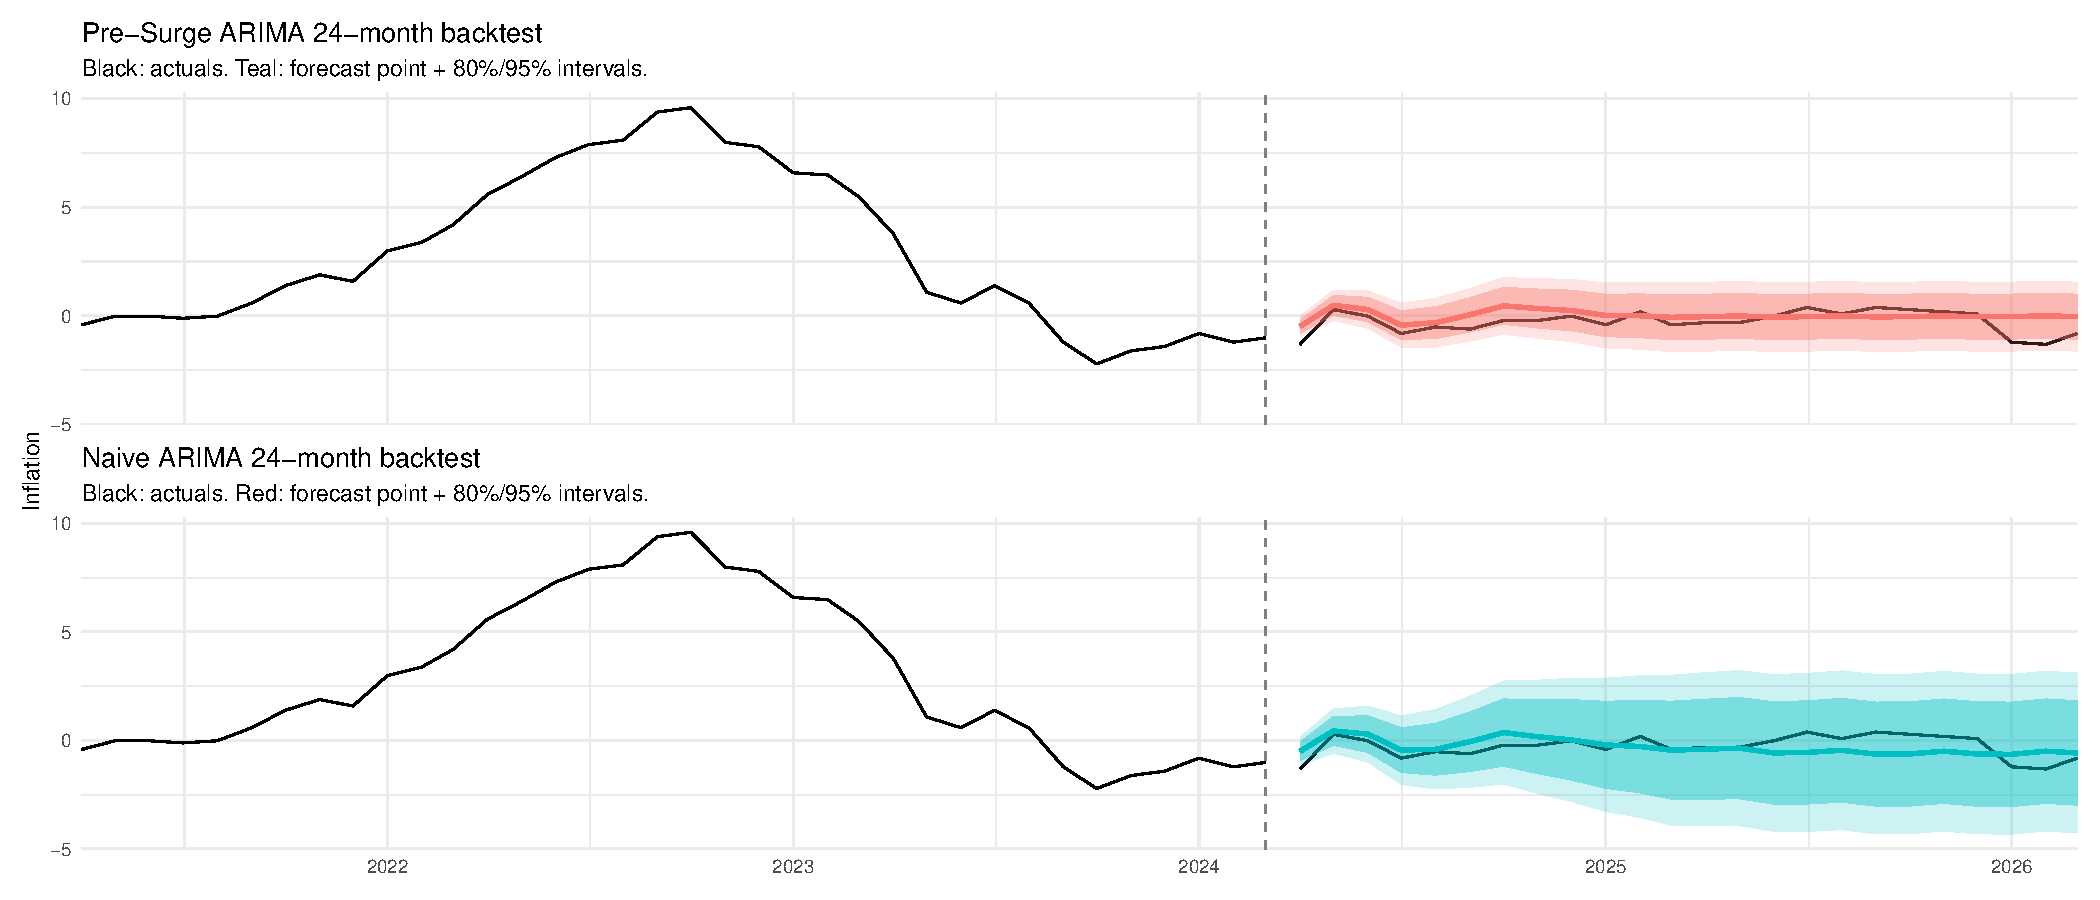
\includegraphics[width=\textwidth]{billeder/arima_forecasts.pdf}
\caption{De-meaned forecast vs.\ actual Danish inflation from 2024}
\label{fig:arima_excl_covid}
\end{figure}



\section{Dynamic Regression Models}
\paragraph{Phillips Curve Model}

AICc-based selection via \texttt{auto.arima()} identifies an ARIMA$(2,0,3)(0,0,1)_{12}$ error structure for the Phillips Curve dynamic regression, yielding
\begin{equation}
y_t = \mathbf{x}'_t\boldsymbol{\beta} + \eta_t, \qquad
\phi_p(B)\,\eta_t = \Theta_Q(B^{12})\,\theta_q(B)\,\varepsilon_t,
\end{equation}
where $\mathbf{x}_t = (\Delta u^{\text{DK}}_t, \Delta u^{\text{DK}}_{t-1}, \ldots, \Delta u^{\text{DK}}_{t-6})'$ contains the distributed lags of first-differenced Danish unemployment, and $\eta_t$ follows an ARIMA$(2,0,3)(0,0,1)_{12}$ process. The estimated coefficients are reported in table~\ref{tab:phillips_coef}.

Two features of the estimates are notable. First, none of the unemployment coefficients attain conventional significance. The implied $t$-statistics range from $0.27$ to $1.33$ in absolute value, well below the five percent critical value (see Table \ref{tab:phillips_coef_appendix}). Second, while all seven point estimates carry the theoretically expected negative sign - a rise in unemployment reducing inflation pressure - the magnitudes are negligible and statistically indistinguishable from zero. Both features are consistent with the Granger causality results in Section~\ref{sec:granger}, where Danish unemployment was found not to Granger-cause Danish inflation at any tested lag structure.

The Ljung--Box statistic at 24 lags equals $35.17$ ($p = 0.009$), rejecting residual white noise at the five percent level. This indicates that the ARIMA$(2,0,3)(0,0,1)_{12}$ error structure does not fully capture the serial dependence remaining after conditioning on unemployment, pointing to model misspecification. 

Out-of-sample (\ref{fig:phillips_curve_forecast}), the model attains an RMSE of $0.552$ and MAE of $0.490$ over the 24-month test period, noticeably worse than the pre-surge ARIMA benchmark ($RMSE = 0.462$ vs. $0.552$). The absence of any gain confirms that DK unemployment provides no incremental forecast content for Danish inflation beyond what is already captured by the model's own ARIMA error dynamics. Taken together, the insignificant unemployment coefficients, the residual autocorrelation, and the absence of out-of-sample improvement constitute a joint rejection of the domestic Phillips Curve hypothesis for Danish inflation over the estimation period.


\begin{table}[H]
\centering
\caption{Model 3 (Phillips Curve) coefficient estimates}
\small{
\begin{tabular*}{\textwidth}{@{\extracolsep{\fill}}lccccccc}
\hline \hline
\rule{0pt}{12pt}\textbf{Parameter} & AR(1) & AR(2) & MA(1) & MA(2) & MA(3) & SMA(1) & Intercept \\[4pt]
\hline
\rule{0pt}{12pt}\textbf{Estimate} & $1.847$ & $-0.855$ & $-0.675$ & $-0.182$ & $0.214$ & $-0.635$ & $1.807$ \\[4pt]
\textbf{Std. err}                  & $(0.053)$ & $(0.052)$ & $(0.073)$ & $(0.062)$ & $(0.064)$ & $(0.054)$ & $(0.295)$ \\[4pt]
\hline
\rule{0pt}{12pt}\textbf{Parameter} & $\Delta u^{\text{DK}}_{t}$ & $\Delta u^{\text{DK}}_{t-1}$ & $\Delta u^{\text{DK}}_{t-2}$ & $\Delta u^{\text{DK}}_{t-3}$ & $\Delta u^{\text{DK}}_{t-4}$ & $\Delta u^{\text{DK}}_{t-5}$ & $\Delta u^{\text{DK}}_{t-6}$ \\[4pt]
\hline
\rule{0pt}{12pt}\textbf{Estimate} & $-0.011$ & $-0.033$ & $-0.027$ & $-0.025$ & $-0.053$ & $-0.048$ & $-0.006$ \\[4pt]
\textbf{Std. err}                  & $(0.022)$ & $(0.036)$ & $(0.041)$ & $(0.038)$ & $(0.040)$ & $(0.036)$ & $(0.022)$ \\[4pt]
\hline \hline
\multicolumn{8}{l}{\rule{0pt}{12pt}\footnotesize $\hat{\sigma}^2 = 0.105$,\;
AICc $= 221.6$,\; BIC $= 276.9$.}
\end{tabular*}
}
\label{tab:phillips_coef}
\end{table}






\paragraph{GETS Variable Selection Model}

The GUM included a constant, AR lags 1 to 6 of Danish inflation, contemporaneous and six lags of first-differenced Danish unemployment ($\Delta u^{\text{DK}}_{t-k}$, $k = 0,\ldots,6$), contemporaneous and six lags of EU27 inflation ($ \pi^{\text{EU}}_{t-k}$, $k = 0,\ldots,6$), and a bounded surge dummy equal to one from April 2021 to July 2023 and zero otherwise. The surge dummy was included as a selectable regressor, so GETS could freely eliminate it if the data did not support it.

After GETS reduction, all six lags of first-differenced Danish unemployment were eliminated as statistically insignificant, consistent with the Granger causality results in Section~\ref{sec:granger}. The surge dummy was likewise eliminated ($p = 0.292$ in the GUM), indicating that the EU27 inflation channel already absorbs the co-movement during the 2021-2023 surge without requiring a separate level correction. The full GUM estimates are reported in Table~\ref{tab:gum_coef} in the appendix. The retained specification contains a constant, AR lags 1, 3, and 6 of Danish inflation, and the contemporaneous change in EU27 inflation, with full coefficient estimates reported in Table~\ref{tab:model4_coef}.


The contemporaneous EU27 inflation change is highly significant ($t = 8.28$, $p < 0.001$), confirming the ERM\,II spillover channel. The AR(3) term is retained despite not individually clearing the five percent threshold ($p = 0.354$), a known property of the GETS path-search: a regressor survives if removing it in any explored elimination path worsens residual diagnostics or destabilises other retained coefficients. The Ljung--Box test at $\ell = 24$ lags yields $p = 0.678$, so we fail to reject residual white noise. The ARCH(1) test yields $p = 0.035$, rejecting homoskedasticity at the five percent level; heteroskedasticity-robust (White) standard errors are used throughout to ensure valid inference.

\begin{table}[H]
\centering
\caption{Model 4 (GETS) coefficient estimates}
\small{
\begin{tabular*}{\textwidth}{@{\extracolsep{\fill}}lccccc}
\hline \hline
\rule{0pt}{12pt}\textbf{Parameter} & Const & AR(1) & AR(3) & AR(6) &
$\pi^{\text{EU}}_{t}$ \\[4pt]
\hline
\rule{0pt}{12pt}\textbf{Estimate} & $0.074$ & $0.973$ & $0.068$ & $-0.098$ &
$0.716$ \\[4pt]
\textbf{Std. err} & $(0.035)$ & $(0.059)$ & $(0.073)$ & $(0.072)$ &
$(0.086)$ \\[4pt]
\hline \hline
\multicolumn{6}{l}{\rule{0pt}{12pt}\footnotesize $\hat{\sigma}^2 = 0.113$,\;
BIC $= 198.7$,\; $R^2 = 0.971$.}
\end{tabular*}
}
\label{tab:model4_coef}
\end{table}



The residual histogram in Figure \ref{fig:gets_residuals} further reveals a distribution with a sharper peak and heavier tails than a normal distribution would produce, suggesting that the normality assumption underlying asymptotic t-statistics may not hold strictly in finite samples. Significance statements for individual coefficients should therefore be interpreted with caution. The White-robust standard errors already address heteroskedasticity, which is the most consequential source of misspecification for inference, but non-normality of residuals remains a caveat.

Out-of-sample, the model attains an RMSE of $0.546$ and MAE of $0.491$ over the 24-month test period, with a mean error of $0.238$, indicating a small systematic over-prediction. This is noticeably worse than the pre-surge ARIMA benchmark ($\text{RMSE} = 0.462$, $\text{MAE} = 0.351$), indicating that the EU27 spillover channel is highly informative in-sample but fails to translate into out-of-sample forecast improvements relative to the benchmark. The elimination of both unemployment and the surge dummy by GETS provides a direct answer to the Phillips curve question: neither domestic labour market conditions nor a structural break correction improve upon the inflation dynamics already explained by autoregressive lags and contemporaneous EU27 inflation.



% -------------------------------------------------------
\section{Model Comparison}
% -------------------------------------------------------
Table~\ref{tab:model_comparison} summarises the out-of-sample forecast performance and in-sample fit statistics across all estimated models.

\begin{table}[H]
\centering
\caption{Model comparison: in-sample fit and out-of-sample forecast accuracy}
\small{
\begin{tabular*}{\textwidth}{@{\extracolsep{\fill}}lccccc}
\hline \hline
\rule{0pt}{12pt}\textbf{Model} & \textbf{AICc} & \textbf{BIC} &
$\hat{\sigma}^2$ & \textbf{RMSE} & \textbf{MAE} \\[4pt]
\hline
\rule{0pt}{12pt}Naive ARIMA$(4,0,5)(0,0,1)_{12}$           & 205.36 & 244.31 & 0.112 & 0.554 & 0.464 \\[4pt]
\rule{0pt}{12pt}Pre-Surge ARIMA$(4,0,2)(0,0,1)_{12}$       &  14.27 &  41.60 & 0.058 & 0.462 & 0.351 \\[4pt]
\rule{0pt}{12pt}Phillips Curve ARIMA$(2,0,3)(0,0,1)_{12}$  & 221.6  & 276.9  & 0.105 & 0.552 & 0.490 \\[4pt]
\rule{0pt}{12pt}GETS Dynamic Regression                     & 180.8  & 198.7  & 0.113 & 0.546 & 0.491 \\[4pt]
\hline \hline
\multicolumn{6}{l}{\rule{0pt}{12pt}\footnotesize RMSE and MAE evaluated
over the 24-month out-of-sample test period.}
\end{tabular*}
}
\label{tab:model_comparison}
\end{table}
Several patterns emerge from the comparison. First, the pre-surge ARIMA dominates the naive specification on every reported metric: its residual variance is roughly half ($\hat{\sigma}^2 = 0.058$ vs.\ $0.112$), and its out-of-sample RMSE is substantially lower ($0.462$ vs.\ $0.554$), with a matching reduction in MAE ($0.351$ vs.\ $0.464$). The in-sample AICc improvement is substantial, reflecting the cost the naive model incurs by forcing its parameter estimates to accommodate the pandemic shock. This confirms the conclusion from Section~\ref{sec:arima} that the additional MA components in the naive specification are an artefact of contaminated estimation rather than genuine ARMA complexity.

Second, the Phillips Curve model provides no forecast improvement over the pre-surge ARIMA benchmark despite conditioning on six lags of unemployment. Its RMSE of $0.552$ exceeds the ARIMA, and its residual autocorrelation, rejected at the five percent level, signals that the ARIMA$(2,0,3)(0,0,1)_{12}$ error structure is insufficient once unemployment is included as a regressor. The Phillips Curve specification therefore adds neither statistical nor economic content. The unemployment coefficients carry the theoretically expected negative sign, none attain conventional
significance, and the model's in-sample AICc of $221.6$ is the highest across all specifications, penalising its additional parameters.

Third, the GETS procedure confirms the irrelevance of domestic unemployment by eliminating all six lags during reduction. The surge dummy, included as a selectable regressor, was likewise eliminated ($p = 0.292$ in the GUM), indicating that EU27 inflation already absorbs the co-movement during the 2021--2023 surge without requiring a separate level correction. The retained model contains only AR lags 1, 3, and 6 alongside contemporaneous EU27 inflation, confirming the ERM\,II spillover channel as the sole empirically relevant external driver of Danish inflation. The Ljung--Box test at $\ell = 24$ lags yields $p = 0.678$, so we fail to reject residual white noise. The ARCH(1) test yields $p = 0.035$, rejecting homoskedasticity at the five percent level; heteroskedasticity-robust (White) standard errors are used throughout, ensuring that $t$-statistics and confidence intervals remain valid despite non-constant error variance due to the COVID shock. 


Taken together, the comparison points to a clear hierarchy. The pre-surge ARIMA establishes that a correctly specified univariate model already captures most of the forecastable variation in Danish inflation. Adding domestic unemployment, as the Phillips Curve prescribes, yields no improvement. The GETS approach corroborates this conclusion and identifies contemporaneous
EU27 inflation as the only external regressor with genuine incremental in-sample content, yet its out-of-sample RMSE of $0.546$ remains above the univariate benchmark's $0.462$. The domestic Phillips Curve relationship, as estimated here, is not a reliable feature of Danish inflation
dynamics over the sample period.

% % -------------------------------------------------------
% \section{TSCV Robustness Check}
% % -------------------------------------------------------

% Time Series Cross-Validation over the full sample yields an RMSE of $0.399$ 
% and MAE of $0.274$ for the ARIMA baseline, based on one-step-ahead forecasts 
% averaged across all expanding windows. These figures are lower than the fixed 
% test set results, which is expected since one-step-ahead errors are inherently 
% smaller than 24-step-ahead errors. The TSCV results confirm that the ARIMA 
% model produces consistent and stable forecasts across the full sample, 
% reinforcing its position as the strongest performing model in this analysis.